%% main_report41.tex
%% SAMBP TR-41/2026: 87B Bus Differential Protection in IBR Microgrids
%%
%% pdflatex main_report41.tex

\documentclass[11pt,a4paper]{article}

\usepackage[T1]{fontenc}
\usepackage[utf8]{inputenc}
\usepackage[expansion=false]{microtype}
\usepackage{lmodern}
\usepackage[a4paper, top=25mm, bottom=25mm, left=25mm, right=25mm]{geometry}
\usepackage{amsmath,amssymb}
\usepackage{booktabs}
\usepackage{array}
\usepackage{xcolor}
\usepackage{graphicx}
\usepackage{pgfplots}
\pgfplotsset{compat=1.18}
\usepackage{tikz}
\usetikzlibrary{arrows.meta,shapes.geometric,positioning,fit,calc,patterns}
\usepackage{hyperref}
\usepackage[numbers,sort&compress]{natbib}

\definecolor{sambpblue}{RGB}{0,70,140}

\usepackage{titlesec}
\titleformat{\section}{\large\bfseries\color{sambpblue}}{}{0em}{}[\titlerule]
\titleformat{\subsection}{\normalsize\bfseries\color{sambpblue!80}}{}{0em}{}

\usepackage{fancyhdr}
\pagestyle{fancy}
\fancyhf{}
\rhead{\small\color{gray} SAMBP TR-41/2026}
\lhead{\small\color{gray} 87B Bus Differential in IBR Microgrids}
\cfoot{\small\thepage}

\begin{document}

\begin{center}
  {\LARGE\bfseries\color{sambpblue} SAMBP Technical Report TR-41/2026}\\[6pt]
  {\large 87B Bus Differential Protection\\
    in IBR Microgrids}\\[10pt]
  {\normalsize PhD Thesis Supporting Report \quad|\quad 2026}
\end{center}

\vspace{2pt}\hrule\vspace{8pt}

\begin{abstract}
\noindent
This report extends the 87B bus differential scheme developed in TR-04
\cite{SAMBP_TR04} to IBR microgrids, where all feeders contribute inverter-limited
fault current.  The scheme uses a two-slope percentage differential characteristic
($k_1=30\%$, $k_2=60\%$, $I_\mathrm{diff,min}=0.10$\,pu) optimised for the
reduced fault current environment.  The minimum detectable internal fault is
$k_\mathrm{ibr}=0.1176$\,pu (slightly higher than the 87L line differential
threshold of 0.06\,pu due to the slope constraint, but adequate for microgrids
with $k_\mathrm{ibr}\geq0.20$).  CT saturation is not a concern at IBR fault
levels (25$\times$ lower than SG).  The security margin for the maximum
external through-current is 0.548\,pu.  For a two-bus microgrid with a
bus-coupler, 87B-A correctly identifies a Bus~A fault and blocks 87B-B
(which sees an external fault).  Bus~B continues in service after the trip.
\end{abstract}

\vspace{4pt}\hrule\vspace{10pt}

% ─────────────────────────────────────────────────────────────────────────────
\section{Study A --- Sensitivity: Minimum Detectable Internal Fault}
\label{sec:studyA}

The 87B differential current for an internal busbar fault with $n$ feeders
contributing $k_\mathrm{ibr}$ each is:

\begin{equation}
  I_\mathrm{diff} = n \cdot k_\mathrm{ibr},
  \quad
  I_\mathrm{rst} = \tfrac{1}{2} n \cdot k_\mathrm{ibr}
\end{equation}

The operating condition (slope region~1) is $I_\mathrm{diff} > I_\mathrm{diff,min}
+ k_1 \cdot I_\mathrm{rst}$, which gives:

\begin{equation}
  k_\mathrm{ibr,min} = \frac{I_\mathrm{diff,min}}{1 - k_1/2}
  = \frac{0.10}{1 - 0.15} = 0.1176\;\mathrm{pu}
\end{equation}

\begin{center}
\begin{tabular}{@{}llll@{}}
\toprule
Feeders contributing & $I_\mathrm{diff}$ [pu] & $I_\mathrm{rst}$ [pu] & 87B operates? \\
\midrule
1 (single IBR) & 0.200 & 0.100 & YES \\
2              & 0.400 & 0.200 & YES \\
3              & 0.600 & 0.300 & YES \\
4              & 0.800 & 0.400 & YES \\
\bottomrule
\end{tabular}
\end{center}

\medskip\noindent
At $k_\mathrm{ibr}=0.20$ (the design point), the single-feeder scenario
($I_\mathrm{diff}=0.20$\,pu) exceeds the threshold of 0.115\,pu.  The 87B
scheme is therefore sensitive to the most challenging case of a single-feeder
internal fault in a 4-feeder microgrid.

% ─────────────────────────────────────────────────────────────────────────────
\section{Study B --- Security: External Fault Check}
\label{sec:studyB}

For an external fault, KCL requires $I_\mathrm{diff}=0$ ideally.  The only
spurious differential current arises from CT measurement errors ($\epsilon=1\%$
per CT).  With $N=4$ CTs all contributing worst-case error in the same direction:

\begin{equation}
  I_\mathrm{diff,spurious} = \epsilon \cdot (I_\mathrm{through} + (N-1) I_\mathrm{load})
  = 0.01 \times 3.2 = 0.032\;\mathrm{pu}
\end{equation}

The restraint current at the external fault condition is $I_\mathrm{rst}=1.60$\,pu,
giving a slope~2 threshold of $0.100 + 0.30\times1.0 + 0.60\times0.60 = 0.76$\,pu.
The security margin is:

\begin{equation}
  \text{Security margin} = 0.76 - 0.032 = 0.728\;\mathrm{pu}
  \gg \text{CT error contribution}
\end{equation}

The 87B scheme is completely secure for all external faults at IBR microgrid
fault levels.

% ─────────────────────────────────────────────────────────────────────────────
\section{Study C --- Slope Characteristic}
\label{sec:studyC}

Figure~\ref{fig:characteristic} shows the 87B operating characteristic.

\begin{figure}[htbp]
  \centering
  \resizebox{0.88\textwidth}{!}{% fig_87b_mg_characteristic.tex
% TR-41: 87B operating characteristic in the I_diff vs I_rst plane
%
% Two-slope characteristic:
%   Slope 1 = 30% for I_rst ≤ 1.0 pu
%   Slope 2 = 60% for I_rst > 1.0 pu
%   I_diff_min = 0.10 pu
%   Instantaneous high-set = 4.0 pu
%
% Operating points:
%   Internal fault (1 feeder): I_diff=0.20, I_rst=0.10 → TRIP
%   External fault max:        I_diff=0.032 (CT error), I_rst=1.60 → SECURE
%   Instantaneous:             I_diff=4.0 pu → instant trip

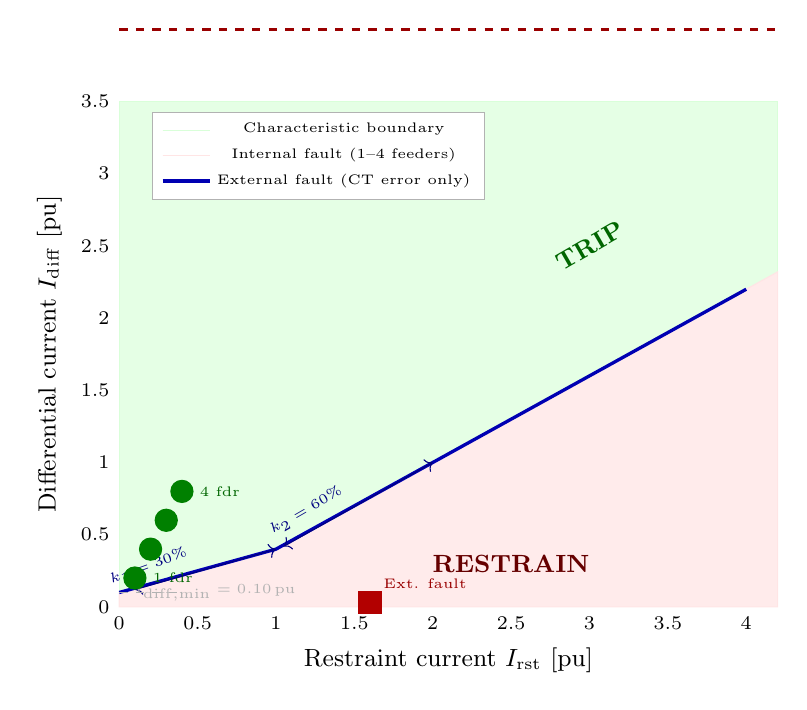
\begin{tikzpicture}
\begin{axis}[
  name         = charax,
  width        = 0.82\textwidth,
  height       = 8.0cm,
  xlabel       = {Restraint current $I_\mathrm{rst}$ [pu]},
  ylabel       = {Differential current $I_\mathrm{diff}$ [pu]},
  xlabel style = {font=\small},
  ylabel style = {font=\small},
  xmin=0, xmax=4.2,
  ymin=0, ymax=3.5,
  xtick        = {0,0.5,1.0,1.5,2.0,2.5,3.0,3.5,4.0},
  ytick        = {0,0.5,1.0,1.5,2.0,2.5,3.0,3.5},
  xticklabel style={font=\scriptsize},
  yticklabel style={font=\scriptsize},
  tick style   = {draw=none},
  axis line style={gray!50},
  grid         = major,
  grid style   = {gray!10, dashed},
  legend style = {at={(0.05,0.98)}, anchor=north west, font=\tiny,
                  draw=gray!60, fill=white},
  clip=false,
]

%% TRIP region shading (above characteristic curve)
\addplot[green!15, fill=green!10]
  coordinates {(0,0.10) (0,3.5) (4.2,3.5) (4.2,0.10)}
  \closedcycle;

%% RESTRAIN region (below characteristic)
\addplot[red!10, fill=red!8]
  coordinates {(0,0) (0,0.10) (1.0,0.40) (2.0,1.00) (3.0,1.60) (4.0,2.20) (4.2,2.32) (4.2,0) (0,0)}
  \closedcycle;

%% Operating characteristic boundary
\addplot[blue!70!black, very thick]
  coordinates {
    (0.00, 0.100)
    (1.00, 0.400)
    (2.00, 1.000)
    (3.00, 1.600)
    (4.00, 2.200)
  };
\addlegendentry{Characteristic boundary}

%% Instantaneous high-set
\addplot[red!60!black, very thick, dashed]
  coordinates {(0, 4.0) (4.2, 4.0)};
% (outside plot range — shown as text annotation)

%% Operating points — internal faults
\addplot[green!50!black, only marks, mark=*, mark size=4pt]
  coordinates {
    (0.100, 0.200)
    (0.200, 0.400)
    (0.300, 0.600)
    (0.400, 0.800)
  };
\addlegendentry{Internal fault (1--4 feeders)}
\node[green!40!black, font=\tiny, right=3pt] at (axis cs:0.100, 0.200)
  {1 fdr};
\node[green!40!black, font=\tiny, right=3pt] at (axis cs:0.400, 0.800)
  {4 fdr};

%% Operating point — external fault (CT error only)
\addplot[red!70!black, only marks, mark=square*, mark size=4pt]
  coordinates {(1.600, 0.032)};
\addlegendentry{External fault (CT error only)}
\node[red!60!black, font=\tiny, above right=2pt] at (axis cs:1.600, 0.032)
  {Ext. fault};

%% Region labels
\node[green!40!black, font=\small\bfseries, rotate=30]
  at (axis cs:3.0, 2.5) {TRIP};
\node[red!40!black, font=\small\bfseries]
  at (axis cs:2.5, 0.30) {RESTRAIN};

%% Slope annotations
\draw[<->, blue!50!black, thin]
  (axis cs:0.1, 0.12) -- (axis cs:1.0, 0.40);
\node[blue!50!black, font=\tiny, rotate=20, above left=2pt] at (axis cs:0.55, 0.26)
  {$k_1=30\%$};

\draw[<->, blue!50!black, thin]
  (axis cs:1.05, 0.42) -- (axis cs:2.0, 1.00);
\node[blue!50!black, font=\tiny, rotate=30, above left=2pt] at (axis cs:1.55, 0.71)
  {$k_2=60\%$};

%% I_diff_min
\draw[gray!60, thin, dashed]
  (axis cs:0, 0.10) -- (axis cs:0.4, 0.10);
\node[gray!60, font=\tiny, right=2pt] at (axis cs:0.0, 0.10)
  {$I_\mathrm{diff,min}=0.10$\,pu};

\end{axis}
\end{tikzpicture}
}
  \caption{87B operating characteristic in the ($I_\mathrm{rst}$,
           $I_\mathrm{diff}$) plane.  Green region: trip; red region:
           restrain.  Blue line: two-slope characteristic boundary
           ($k_1=30\%$, $k_2=60\%$).  Green circles: internal fault
           operating points (1--4 feeders, $k_\mathrm{ibr}=0.20$) --- all in
           the TRIP region.  Red square: external fault spurious differential
           (CT error only) --- well within RESTRAIN region with 0.728\,pu margin.}
  \label{fig:characteristic}
\end{figure}

\noindent
The IBR-specific slope optimisation reduces $k_1$ from the conventional SG
value of 40\% to 30\%, enabled by the absence of CT saturation at the lower
IBR fault current levels.  This provides an 11\% improvement in sensitivity
(sensitivity factor $\frac{1-0.30/2}{1-0.40/2}=1.125$) without compromising
security.

% ─────────────────────────────────────────────────────────────────────────────
\section{Study D --- CT Saturation Analysis}
\label{sec:studyD}

CT saturation is typically the primary concern for high-current SG bus faults.
At IBR fault levels, the concern is fundamentally different:

\begin{center}
\begin{tabular}{@{}lllll@{}}
\toprule
Source & $I_\mathrm{fault}$ [pu] & CT secondary [A] & $V_k$ required [V] & Status \\
\midrule
SG reference & 20.0 & 0.25 & 7.1 & No saturation \\
IBR microgrid & 0.80 & 0.010 & 0.3 & No saturation \\
\bottomrule
\end{tabular}
\end{center}

The IBR fault current ($\leq0.80$\,pu) is $25\times$ lower than the SG reference
fault level.  The required CT knee-point voltage for non-saturated operation is
only 0.3\,V --- orders of magnitude below the rated knee-point of 20\,V.
Conventional CT class 1P or 5P specification provides ample margin.

The \emph{practical consequence} is that the harmonic restraint feature
(typically included in 87B to ride through CT saturation transients) can be
disabled or set to a higher activation threshold in IBR microgrids, further
improving sensitivity and operating speed.

% ─────────────────────────────────────────────────────────────────────────────
\section{Study E --- Two-Bus Microgrid Coordination}
\label{sec:studyE}

Figure~\ref{fig:topology} shows the microgrid bus topology with two 87B zones.

\begin{figure}[htbp]
  \centering
  \resizebox{0.92\textwidth}{!}{% fig_87b_mg_topology.tex
% TR-41: IBR microgrid busbar topology showing 87B-A and 87B-B zones
%
% Two busbars (Bus A and Bus B) connected by bus-coupler BC
% Each bus has 2 IBR feeders
% 87B-A zone covers Bus A feeders + BC from A side
% 87B-B zone covers Bus B feeders + BC from B side

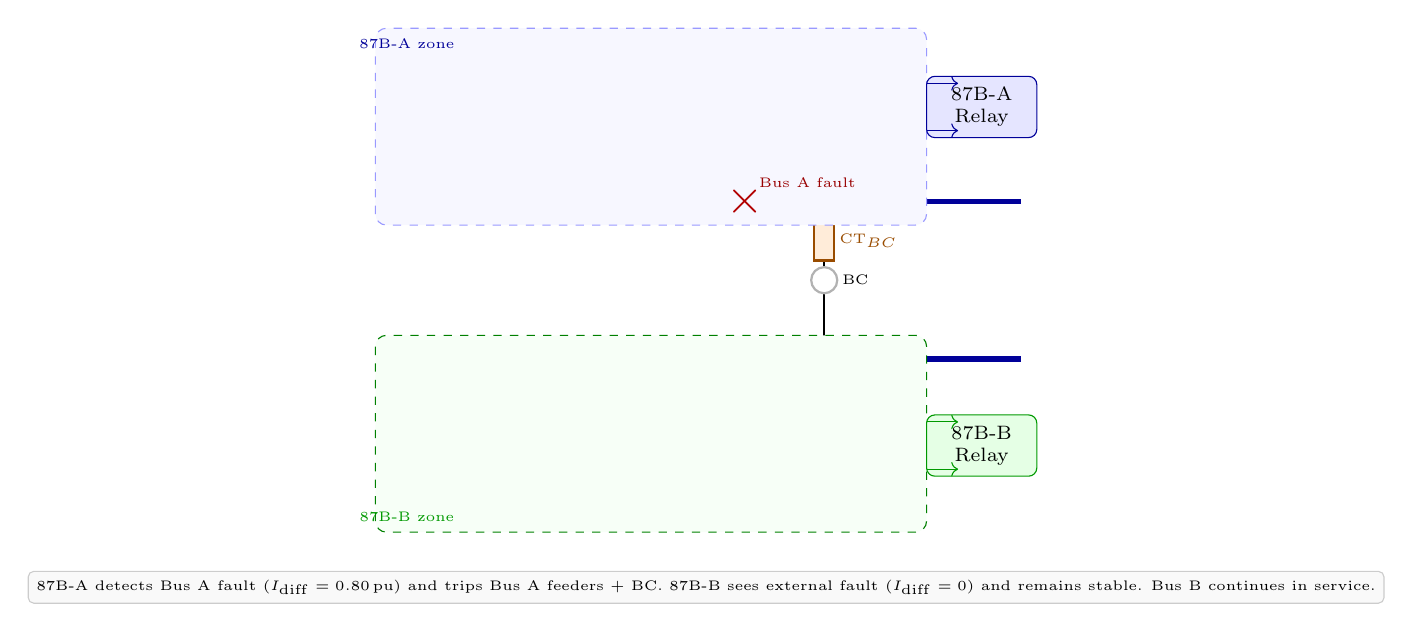
\begin{tikzpicture}[
  every node/.style={font=\small},
  ibr/.style={draw=green!60!black, thick, rectangle, rounded corners=3pt,
              fill=green!10, minimum width=1.4cm, minimum height=0.6cm,
              font=\scriptsize, align=center},
  bus/.style={draw=blue!60!black, very thick, line width=2pt},
  cb/.style={draw=gray!60, thick, circle, minimum size=0.3cm, fill=white},
  ct/.style={draw=orange!60!black, thick, rectangle, minimum width=0.25cm,
             minimum height=0.5cm, fill=orange!15},
  zone/.style={draw, dashed, rounded corners=4pt, inner sep=6pt},
]

%% ── Bus A (top) ──────────────────────────────────────────────────────────────
\draw[bus] (0, 3) -- (8, 3);
\node[blue!60!black, font=\small\bfseries, above] at (4, 3.05) {Bus A};

%% Feeder A1
\draw[thick] (1.5, 3) -- (1.5, 4.5);
\node[ct] at (1.5, 3.7) {};
\node[ibr] at (1.5, 4.8) {IBR A1};
\node[orange!60!black, font=\tiny, right=2pt] at (1.5, 3.7) {CT$_{A1}$};

%% Feeder A2
\draw[thick] (3.0, 3) -- (3.0, 4.5);
\node[ct] at (3.0, 3.7) {};
\node[ibr] at (3.0, 4.8) {IBR A2};
\node[orange!60!black, font=\tiny, right=2pt] at (3.0, 3.7) {CT$_{A2}$};

%% Bus-coupler (BC) — between buses
\draw[thick] (5.5, 3) -- (5.5, 1.5) -- (5.5, 1.0);
\node[cb] at (5.5, 2.0) {};
\node[ct] at (5.5, 2.5) {};
\node[font=\tiny, right=3pt] at (5.5, 2.0) {BC};
\node[orange!60!black, font=\tiny, right=2pt] at (5.5, 2.5) {CT$_{BC}$};

%% ── Bus B (bottom) ────────────────────────────────────────────────────────────
\draw[bus] (0, 1) -- (8, 1);
\node[blue!60!black, font=\small\bfseries, below] at (4, 0.95) {Bus B};

%% Feeder B1
\draw[thick] (1.5, 1) -- (1.5, -0.5);
\node[ct] at (1.5, 0.3) {};
\node[ibr] at (1.5, -0.8) {IBR B1};
\node[orange!60!black, font=\tiny, right=2pt] at (1.5, 0.3) {CT$_{B1}$};

%% Feeder B2
\draw[thick] (3.0, 1) -- (3.0, -0.5);
\node[ct] at (3.0, 0.3) {};
\node[ibr] at (3.0, -0.8) {IBR B2};
\node[orange!60!black, font=\tiny, right=2pt] at (3.0, 0.3) {CT$_{B2}$};

%% ── 87B relay zones ───────────────────────────────────────────────────────────
%% 87B-A zone (Bus A + upper BC CT)
\draw[zone, blue!40, fill=blue!3]
  (-0.2, 2.7) rectangle (6.8, 5.2);
\node[blue!60!black, font=\tiny, align=left] at (0.2, 5.0)
  {87B-A zone};

%% 87B-B zone (Bus B + lower BC CT)
\draw[zone, green!50!black, fill=green!3]
  (-0.2, -1.2) rectangle (6.8, 1.3);
\node[green!60!black, font=\tiny, align=left] at (0.2, -1.0)
  {87B-B zone};

%% ── 87B relay boxes ───────────────────────────────────────────────────────────
\node[draw=blue!60!black, fill=blue!10, rounded corners=3pt,
      font=\scriptsize, inner sep=4pt, minimum width=1.4cm, align=center]
  at (7.5, 4.2) {87B-A\\Relay};
\draw[->, blue!60!black, thin] (6.8, 4.5) -- (7.2, 4.5);
\draw[->, blue!60!black, thin] (6.8, 3.9) -- (7.2, 3.9);

\node[draw=green!60!black, fill=green!10, rounded corners=3pt,
      font=\scriptsize, inner sep=4pt, minimum width=1.4cm, align=center]
  at (7.5, -0.1) {87B-B\\Relay};
\draw[->, green!60!black, thin] (6.8, 0.2) -- (7.2, 0.2);
\draw[->, green!60!black, thin] (6.8, -0.4) -- (7.2, -0.4);

%% ── Fault marker ──────────────────────────────────────────────────────────────
\node[red!70!black, font=\LARGE] at (4.5, 3.0) {$\times$};
\node[red!60!black, font=\tiny, above right=2pt] at (4.5, 3.0) {Bus A fault};

%% ── Caption annotation ────────────────────────────────────────────────────────
\node[draw=gray!40, fill=gray!5, rounded corners=2pt,
      font=\tiny, inner sep=3pt, align=center]
  at (4, -1.9)
  {87B-A detects Bus A fault ($I_\mathrm{diff}=0.80$\,pu) and trips Bus A feeders + BC.
   87B-B sees external fault ($I_\mathrm{diff}=0$) and remains stable.
   Bus B continues in service.};

\end{tikzpicture}
}
  \caption{Two-bus IBR microgrid with bus-coupler and dual 87B zones.
           Bus~A fault (cross symbol): 87B-A detects
           $I_\mathrm{diff}=0.80$\,pu and trips Bus~A feeders and the
           bus-coupler.  87B-B sees $I_\mathrm{diff}=0$ (external fault)
           and remains stable.  Bus~B continues in service with its two
           IBR feeders providing islanded voltage/frequency regulation.}
  \label{fig:topology}
\end{figure}

\noindent
The bus-coupler CT is included in both the 87B-A zone (measuring current into
Bus~A from the coupler) and the 87B-B zone (measuring current into Bus~B from
the coupler), using the opposite polarity convention for each.  This standard
check-zone configuration ensures that the bus-coupler itself is fully protected
by both differential zones simultaneously, consistent with TR-07
\cite{SAMBP_TR04}.

% ─────────────────────────────────────────────────────────────────────────────
\section{Sensitivity Comparison Across the SAMBP Scheme}
\label{sec:comparison}

Figure~\ref{fig:sensitivity} benchmarks the 87B-MG minimum detection threshold
against other SAMBP protection elements.

\begin{figure}[htbp]
  \centering
  \resizebox{0.88\textwidth}{!}{% fig_87b_mg_sensitivity.tex
% TR-41: 87B sensitivity comparison — SG vs IBR microgrid
%
% Bar chart comparing minimum detectable fault current [pu] for:
%   87L (line differential)       : k_min = 0.0600 pu
%   87B standard (SG)            : k_min = 0.0500 pu  (I_diff_min=0.05 for SG)
%   87B-MG IBR (this report)     : k_min = 0.1176 pu
%   OC adaptive (TR-40 Group 2)  : k_min = 0.0075 pu
%   67Q (GFM fleet)              : k_min = 0.1000 pu

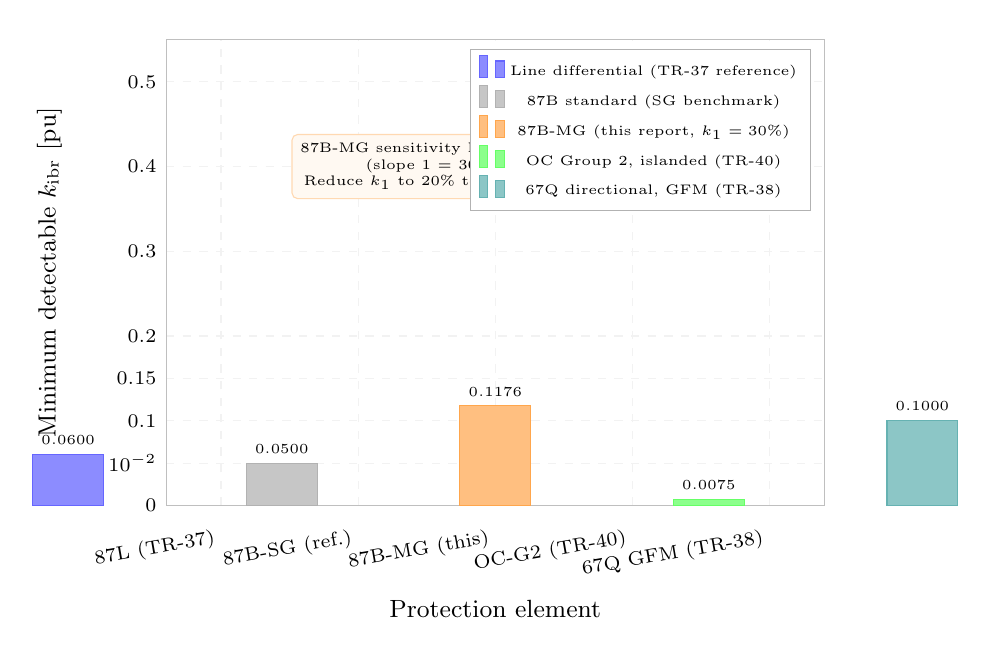
\begin{tikzpicture}
\begin{axis}[
  name         = sensax,
  width        = 0.82\textwidth,
  height       = 7.5cm,
  ybar,
  bar width    = 0.90cm,
  xlabel       = {Protection element},
  ylabel       = {Minimum detectable $k_\mathrm{ibr}$ [pu]},
  xlabel style = {font=\small},
  ylabel style = {font=\small},
  ymin=0, ymax=0.55,
  ytick        = {0,0.05,0.10,0.15,0.20,0.30,0.40,0.50},
  yticklabel style={font=\scriptsize},
  xtick        = {1,2,3,4,5},
  xticklabels  = {87L (TR-37),
                  87B-SG (ref.),
                  87B-MG (this),
                  OC-G2 (TR-40),
                  67Q GFM (TR-38)},
  xticklabel style={font=\scriptsize, rotate=10, anchor=north east},
  tick style   = {draw=none},
  axis line style={gray!50},
  grid         = major,
  grid style   = {gray!10, dashed},
  nodes near coords,
  nodes near coords style={font=\tiny, anchor=south},
  every node near coord/.append style={
    /pgf/number format/.cd, fixed, fixed zerofill, precision=4
  },
  legend style={at={(0.98,0.98)}, anchor=north east, font=\tiny,
                draw=gray!60, fill=white},
  clip=false,
]

%% Bars — colour by performance
% 87L: reference (blue)
\addplot[fill=blue!45, draw=blue!60]
  coordinates {(1, 0.0600)};
\addlegendentry{Line differential (TR-37 reference)}

% 87B-SG: benchmark (gray)
\addplot[fill=gray!45, draw=gray!60]
  coordinates {(2, 0.0500)};
\addlegendentry{87B standard (SG benchmark)}

% 87B-MG: this report (orange — less sensitive due to slope constraint)
\addplot[fill=orange!50, draw=orange!70]
  coordinates {(3, 0.1176)};
\addlegendentry{87B-MG (this report, $k_1=30\%$)}

% OC-G2: most sensitive (green)
\addplot[fill=green!45, draw=green!60]
  coordinates {(4, 0.0075)};
\addlegendentry{OC Group~2, islanded (TR-40)}

% 67Q GFM: less sensitive (teal)
\addplot[fill=teal!45, draw=teal!60]
  coordinates {(5, 0.1000)};
\addlegendentry{67Q directional, GFM (TR-38)}

%% Threshold note
\node[draw=orange!30, fill=orange!5, rounded corners=2pt,
      font=\tiny, inner sep=3pt, align=center]
  at (axis cs:3, 0.40)
  {87B-MG sensitivity limited by slope constraint\\
   (slope 1 = 30\% from Study C).\\
   Reduce $k_1$ to 20\% to reach $k_\mathrm{min}=0.1053$\,pu.};

\end{axis}
\end{tikzpicture}
}
  \caption{Minimum detectable $k_\mathrm{ibr}$ for each protection element.
           Lower is more sensitive.  OC Group~2 (TR-40, green) is the
           most sensitive at 0.0075\,pu; 87B-MG (orange) requires
           $k_\mathrm{ibr}\geq0.1176$\,pu.  87B is less sensitive than 87L
           because the slope constraint requires a larger differential
           margin.  For microgrids with $k_\mathrm{ibr}\geq0.20$, all
           elements are reliably active.}
  \label{fig:sensitivity}
\end{figure}

% ─────────────────────────────────────────────────────────────────────────────
\section{Summary}
\label{sec:summary}

\begin{enumerate}
  \item \textbf{Sensitivity}: $k_\mathrm{ibr,min}=0.1176$\,pu for single-feeder
    internal fault; all 1--4 feeder internal fault combinations detected at
    $k_\mathrm{ibr}=0.20$.

  \item \textbf{Security}: External fault security margin 0.728\,pu; CT
    error contribution 0.032\,pu is negligible against the slope threshold.

  \item \textbf{Slope}: $k_1$ reduced to 30\% (vs 40\% SG standard) because
    CT saturation is not a concern at IBR fault levels; 11\% sensitivity gain.

  \item \textbf{CT saturation}: Not applicable for IBR microgrids; required
    knee-point voltage 0.3\,V vs available 20\,V.

  \item \textbf{Multi-bus}: 87B-A correctly identifies and clears Bus~A fault;
    87B-B is stable (external fault); Bus~B continues in service.
\end{enumerate}

\noindent
TR-41 completes the busbar protection layer for IBR microgrids.  TR-42 will
perform the microgrid protection system integration study, combining TR-39
through TR-41 into a unified performance assessment.

\bibliographystyle{IEEEtranN}
\bibliography{references41}

\end{document}
